\documentclass[12pt]{article}

\usepackage[T2A]{fontenc}
\usepackage[utf8]{inputenc}
\usepackage[russian]{babel}
\usepackage{amsthm, amsmath, amssymb}
\usepackage[russian]{hyperref}
\usepackage{datetime}
\usepackage{cmap}
\usepackage{enumerate}
\usepackage{color}
\usepackage{picture}
\usepackage{graphics}

\title{\textbf{Описание приложения auTimetable}}
\author{Kravchenko Dmitry\\
		Rozplokhas Dmitry}
\date{}

\voffset=-20mm
\textheight=220mm

\hoffset=-10mm
\textwidth=155mm

\def\EPS{\varepsilon}
\def\SO{\Rightarrow}
\def\EQ{\Leftrightarrow}
\def\t{\texttt}
\def\O{\mathcal{O}}

\newlength{\myskip}
\setlength{\myskip}{0.5em}

\begin{document}

\maketitle

\section*{General}
Наше приложение -- электронное расписание для АУ.\\
Перед началом каждой пары присылает нотификацию -- во сколько след. пара, 
что за пара, в каком кабинете.

Видимо, мы сделаем все аккаунты просто с возможностью просмотра и 1 аккаунт --
с возможностью внесения изменений.

Расписание пока, наверно, просто будем хранить в гугл-таблицах. Будет, скажем,
4 таблицы -- на каждый из курсов. Когда человек смотрит ее, то загружаем
на телефон и храним как-нибудь в XML-ке прямо на устройсве. + кнопочка 
"обновить"\,, чтобы, понятно, опять подключиться к сети и загрузить
таблику (т.е. чтобы была возможность смотреть таблицу в offline, а так же
обновлять, в случае чего). Табличка, например, состоит из 5ти колонок
и просто в каждом 12 строчек: название 1го предмета, кабинет, препод, 2го, 
кабинет, препод и т.д. (т.е. на одну пару 3 строки -- предмет, кабинет, ФИО 
препода). Но это так, примерно.

В идеале, потом надо сделать свой сервер, где хранить расписание, и какой-
нибудь веб-клиент с каким-то минимальным ui, чтобы можно было вносить какие-то
изменения (или сделать админский аккаунт прямо внутри приложение и он 
едиственный может вносить изменения (или и то и то, но, боюсь, и 1го-то
можем не успеть)).
\section{Общий вид}
Слева выдвижная (по свайпу) менюшка (как в ВК, например) с пунктами:
\begin{enumerate}
\item
	\textbf{timetable}
\item
	\textbf{contacts}
\item
	\textbf{announcements}
\item
	\textbf{scores}
\end{enumerate}

В правом верхнем углу шестереночка -- меню настроек.

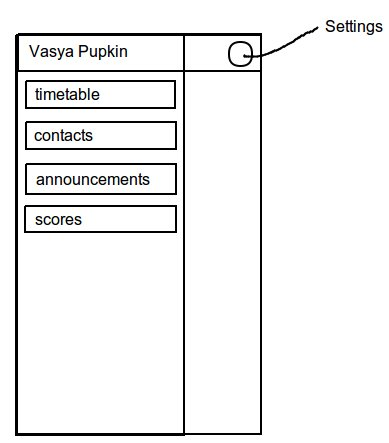
\includegraphics{term3.jpg}

\section{timetable}
Здесь будет само расписание. 

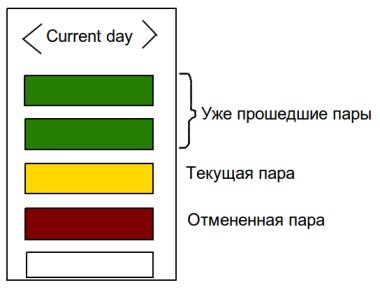
\includegraphics{timetable.jpg}

В каждом прямоугольничке -- название предмета, номер кабинета, ФИО 
преподавателя. В идеале, по клику можно открывать доп. информацию 
типа прикрепленного домашнего задания

\section{contacts}
Контакты всех преподавателей. Изначально нужно выбрать список, каких преподов
хочешь смотреть (по предметам), либо же всех

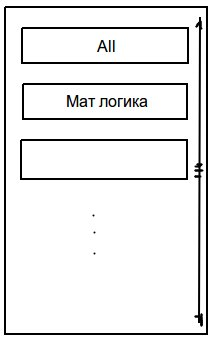
\includegraphics{contacts1.jpg}

Каждый список выглядит примерно так:

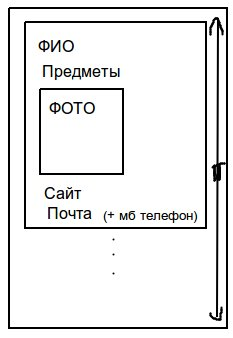
\includegraphics{contacts2.jpg}

вообще, чтобы конкретно так красиво все сделать, наверно, понадобиться сервер
и веб-клиент, чтобы все это добавлять. Но для начала можно так же сделать
тупо в гугл-табличках, примерно как расписание. Типа колонка с такими
строками:\\
ФИО\\
Через запятую, какие предметы ведет\\
Сайт (или прочерк)\\
Почта (или прочерк)

\section{announcements}
Все объявления (по каждому курсу отдельно) в порядке добавления. Они будут 
получаться просто из
google группы. Чтобы их получать, можно запросить разрешение на чтение
почты и просто выводить те сообщение, которые пришли из нужно группы
(название можно просто захардкодить в начале года). Либо же, если эти
группы открыты и любой может читать их обновления -- то можно просто
читать это ботом, без чтения почты владельца устройства. Третий вариант --
создаем бота \texttt{autimetable\_bot@gmail.com}. В начале года его
просто добавляют в новые группы, на него будут приходить сообщения, он будет
это просто высылать на устройства.\\
Просто мы особо не знаем, как эти группы все устроенны, так что точно не можем
сейчас сказать, как будет лучше. Но, думаю, это не так важно -- с этим можно
потом быстро разобраться.

\section{scores}
Таблицы результатов. Если сможем научиться нормально экспортировать из гугл-
таблиц, то будем прям тут показывать, но, как минимум, можно просто ссылочки 
хранить.

\section{settings}
Какие-то настройки. Обязательное: курс и группа. Остальное, если что 
понадобиться, добавим (типа фамилия, имя)

\section*{conclusion}
Т.е. для начала мы просто, видимо, создадим кучу гугл-таблиц, которые 
захардкодим в приложении и будем всю инфу брать из них. 

Если произойдет чудо,
мы быстро разберемся с андроидом, то можно будет написать свой сервер и 
веб-клиент (или хотя бы админский акк в приложении). Сервер, наверно, можно
сделать хотя бы в том же google app engine'e. Мы больше никогда ни с чем 
другим не работали, а там, вроде, относительно просто.

\end{document}
